\section{Analysis and results}
Firstly we have to build a business model canvas for Meta social media
platforms. They all more or less use the same principles and offer the
same experience to their customers, what changes between them is the
actual content published and the target demographic for the platform.
A version could be the picture \ref{fig:fbcanvas}.

\begin{figure}[ht]
  \centering
  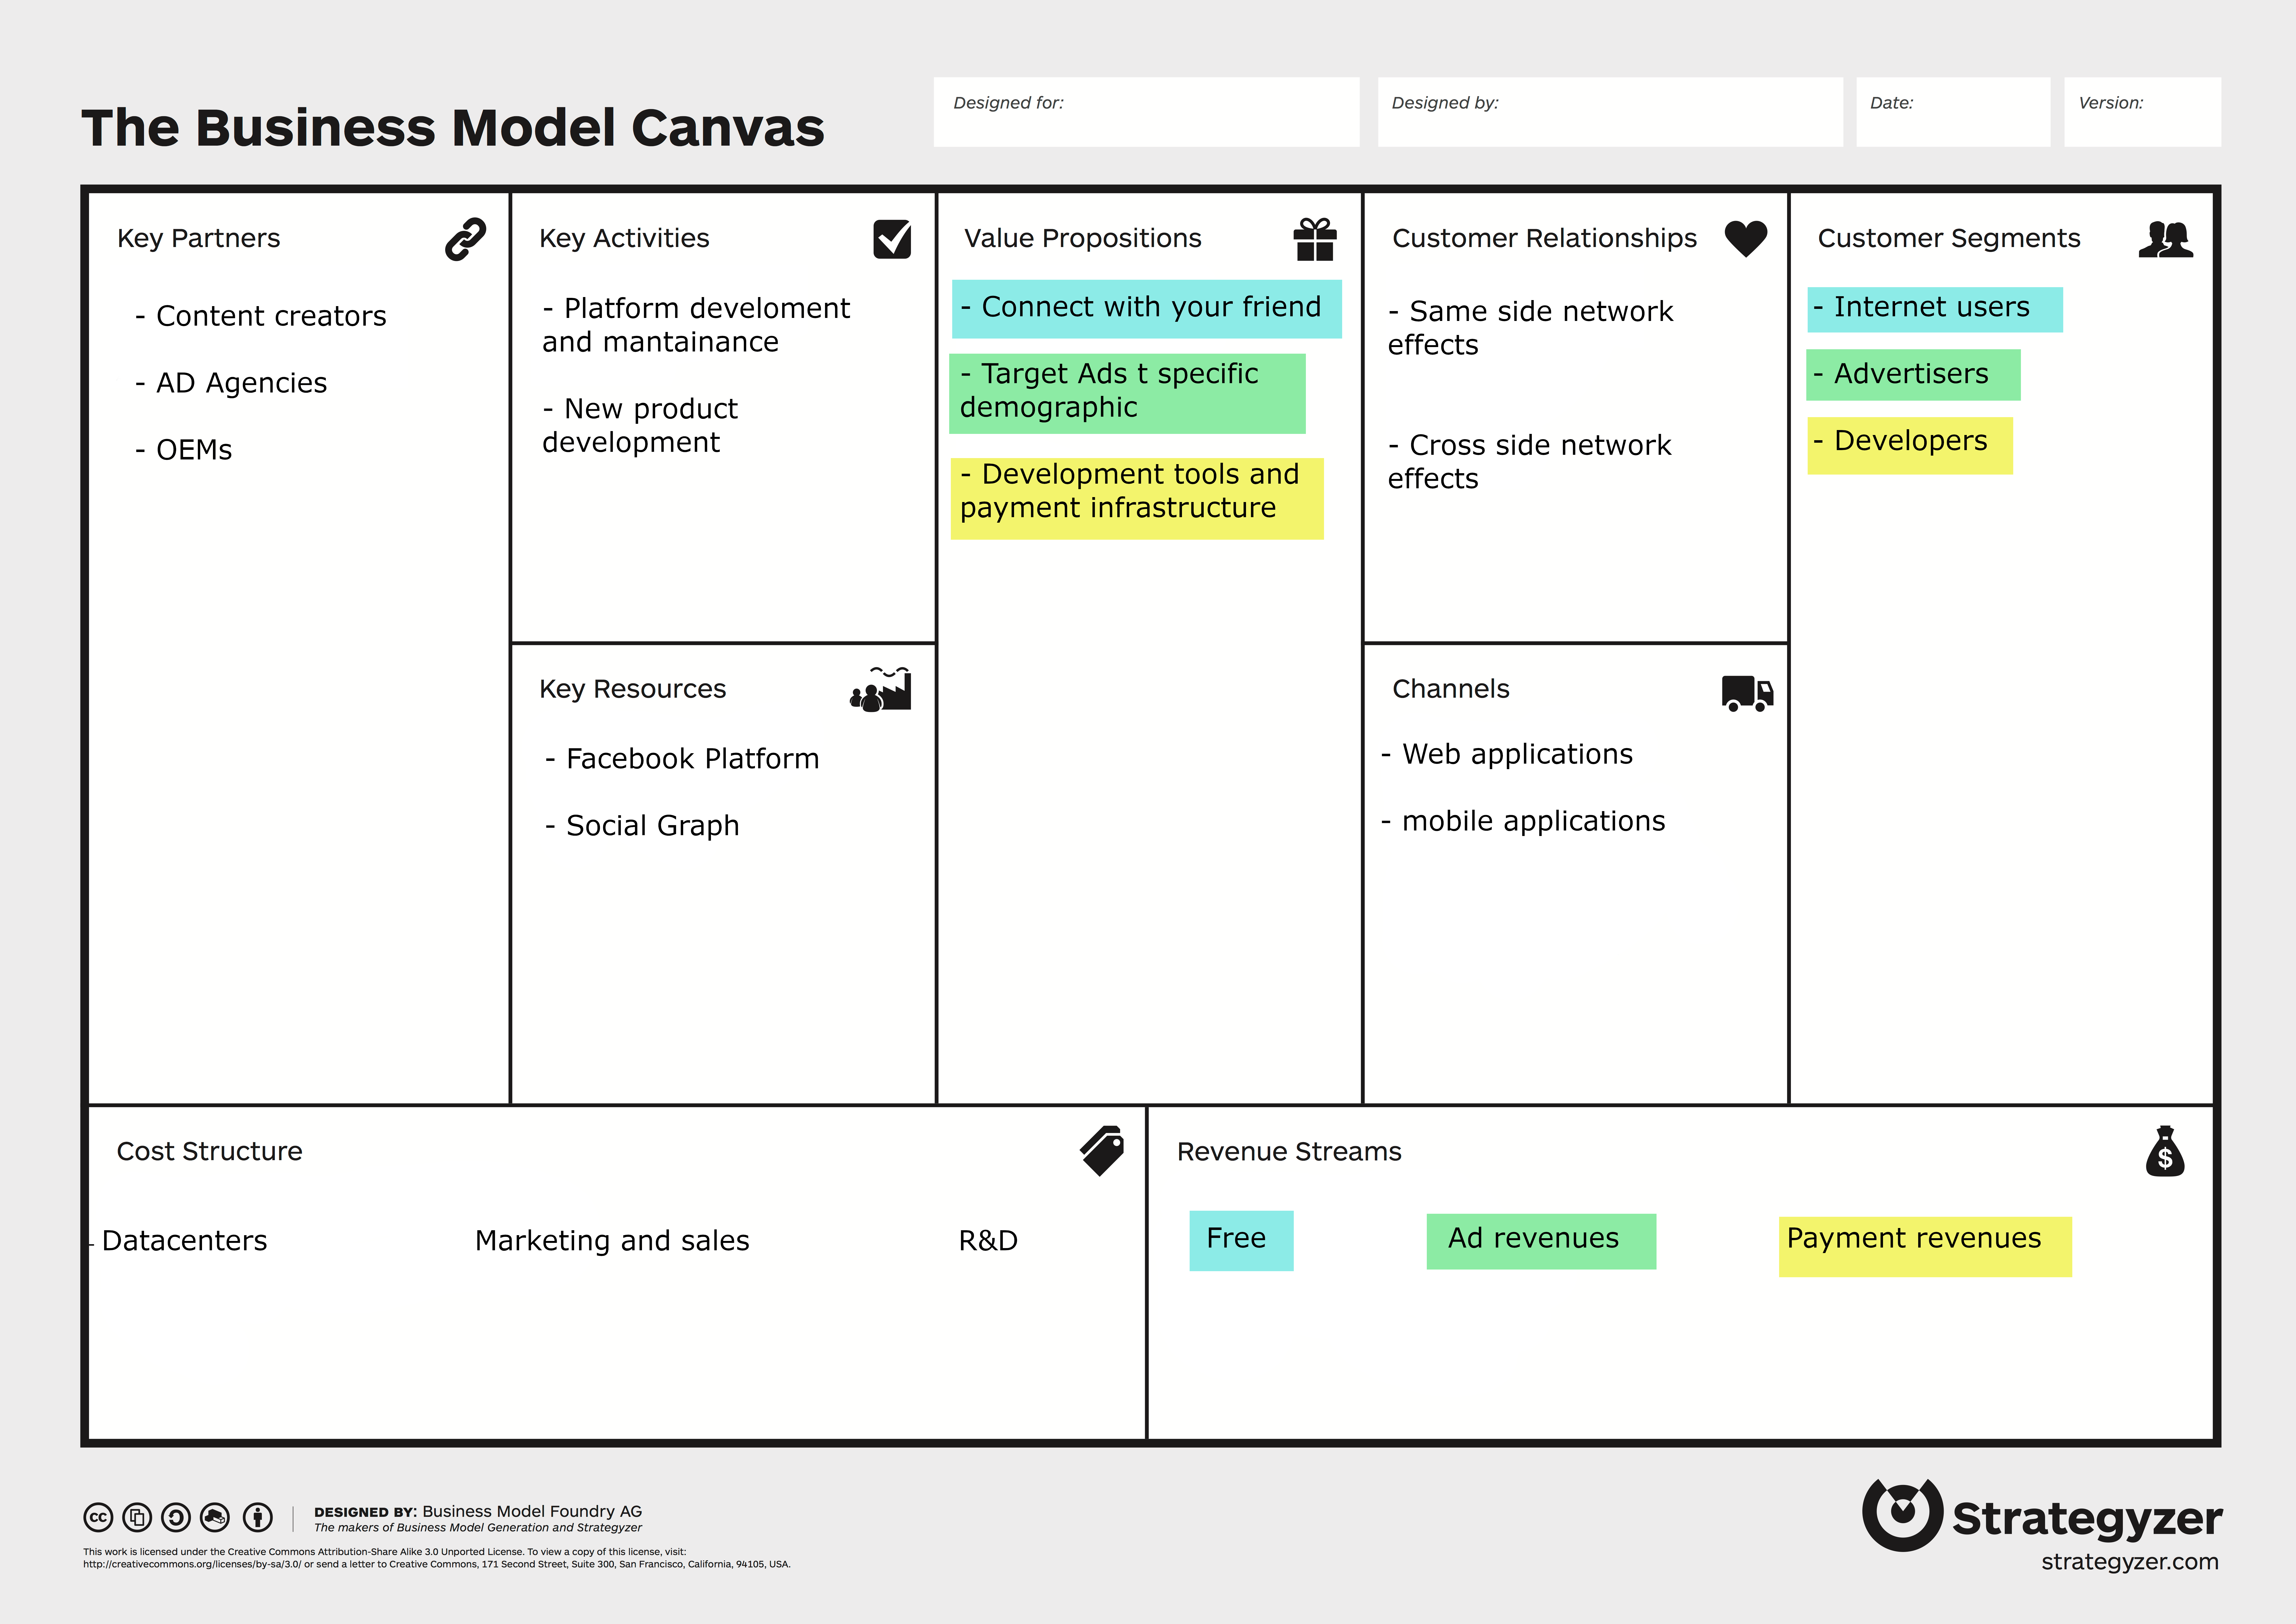
\includegraphics[width=.8\textwidth]{images/fbcanvas.png}
  \caption{Meta social media business model canvas, source: autohr's
    elaboration}
  \label{fig:fbcanvas}
\end{figure}

We'll now explain briefly the business model of facebook trought the
canvas:

\paragraph{Key partners}
These are mainly content creators, Ad agenies and OEMs. Content
creators are important to create appeal to the platform, and attract
more and more users to it, making it an aggregation point for any type
of subculture, enlarging this way the social graph of the platform.

\paragraph{Key activities}
The key activities at meta are the development of their platforms
(mainly instagram and facebook for the focus of this report) and the
development of new products. Meta in fact has other products
(e.g. Oculus and Novi), so one of its core activities is the active
serch of new products.

\paragraph{Key resources}
Within Meta key resources, the only tangible one (but essentially
digital) is its platforms, which demands technological infrastructure.

Aside from that, the other key resources are the network users and
their content production, and the ``Meta'' brand. The active users are
the company's biggest asset. Because, if there aren't users, there is
no audience to view the ads. And to make them engaged, there must be
relevant content, to avoid churn.

\paragraph{Value proposition}
As Meta has three diverse customer segments, each segment will
perceive the brand's value in a different way. That said, let's divide
the value proposition by segment:

\begin{itemize}
\item \textbf{For users}: the greatest benefit is to keep in touch
  with family and friends, via text and picture posting, and by
  interactions through comments and direct messages. This is
  especially relevant for the ones who travel a lot or live far from
  their loved ones. Another advantage is the availability of
  entertainment and information. Meta is useful both for those who
  want to get entertained by the lives of their acquaintances and for
  people who use it as a source of news and current affairs.

\item \textbf{For advertisers}: the possibility of targeted campaigns,
  focused on their particular target audience, has been of great value
  for brands. By achieving greater penetration in its main audience,
  companies also get greater engagement in their customer segment of
  interest. Another relevant point, especially for small businesses or
  young companies is that the tools to advertise on Meta's platofrms
  are quite simple, in the best ``do it yourself'' style, which
  reduces the need to hire someone to develop their own advertising
  content.

\item \textbf{For developers}: Meta is an amazing platform for
  developing apps and games, and it offers a wide range view and
  disclosure. Besides, there is a great network of providers for
  advertisement services.
\end{itemize}

\paragraph{Customer relationships}
Meta's customer relationship is based on its own platforms (this works
for both instagram and facebook), which are very user-friendly, as
they allow users to specify their profile configurations and use, with
no hard time. In addition, Meta has an international sales
organization, that works alongside with marketing and advertising
agencies, to attract advertisers.

\paragraph{Channels of distribution}
It's quite clear that the main distribution channels of Meta are its
own products websites and apps, because that's where users find each
other, and advertisers access their audience. Inside them, the
channels can be divided into Feed, notifications, direct messages, and
stories.

\paragraph{User segments}
\begin{itemize}
\item \textbf{Users}: they are the biggest customer segment of Meta,
  and stand for one-third of the world's population. They are all the
  people who have their profiles in the network and use them to
  interact and communicate with friends and other people with similar
  interests around the globe. They don't pay Meta anything and, thus,
  they are not directly responsible for the business revenue. However,
  they are the basis who make Meta's platforms interesting for the
  ones who do pay.

\item \textbf{Business and Advertisers}: this is the segment involved
  in Meta's revenue. It encompasses all the brands and businesses that
  advertise in the social networks. They pay to have ads of their
  products and services on the platform, which, from its side, offers
  a more qualified audience. Due to the information Meta collects from
  its users, the company is able to target advertisement into its
  platform, allowing brands and businesses to have their ads viewed by
  its target audience. Anyway, although these are the revenue
  providers, they will only keep their interest as long as the
  non-paying user base is wide and qualified.

\item \textbf{Developers}: it's the smallest customer segment and it
  includes the ones who develop apps and games through Facebook's
  platform.
\end{itemize}

\paragraph{Cost structure}
The biggest share of Meta's cost structure revolves around platform
maintenance and its billions of users' data storage. Besides, there is
user CAC (cost of acquisition) by delivering tools that foster user
engagement, research and development investment, marketing and
advertising, customer support, and all the regular general and
administrative expenses of a worldwide company.

\paragraph{Rvenue streams}
Advertisement, commissions on games played and products sold on the
platform, sales of private social network services to businesses, and
sales of products (like Oculus virtual reality device).

\subsection{Main point and results}
The main point of this canvas is that there are three main customers
of Meta's platforms. Users, who use the platform for free, and provide
no direct revenue stream for the company. These customers however are
essential to the platforms, since they rapresent the real value that
is later sold to the other two clients. This means that is vital to
the platform to mantain a good overall relashionship with its
users. In this scenario a problem has emerged in the last decade. From
\cite{art:fortuna2018survey} we can see how the recognition of HS has
become more and more a problem that social platform had to face in the
last years, and how more and more literature has been published about
it. Meta, with its two main products Instagram and Facebook is no
exception. This particular phenomena becomes a problem when the
backbone AI of the platform is trained in order to maximize angagment,
and for some users, HS is the content that keeps them inside
of Meta's social platforms. But HS is controversial, and nor
advertisers, nor some users want to see it. For the company has become
more and more of a problem that of investors and users opting out of
the platform for this very reason.

Here starts the journey of another AI trained to remove HS
from the platform. Over the years the platform has used various
approach to model the different systems to tackle HS, and
recently a new model composed by few-shot-learners has emerged. The
main problem is that these systems have to evolve rapidly, since the
laguage is doing so naturally. Traditional systems evolve thanks to
new data in a matter of months, but few-shot-learners require less
time, and the method developed by Meta requires even less time,
outperforming other comparabel FSLs up to 55\%, and 12\% in averge
\cite[pp.~5-8]{art:entailing}.

In the business model we presented, this innovation interests users
and advertisers. Users because it helps to create a better social
community inside of the platform for everyone to live in, discouraging
disengagement due to HS. Advertisers since generally these
customers dont like teir products associated to HS, and when
the automatic systems arrociate an advertiser to HS content this tends
to leave the platform, diminuishing the revenue stream that it brings.

\begin{figure}[ht]
  \centering 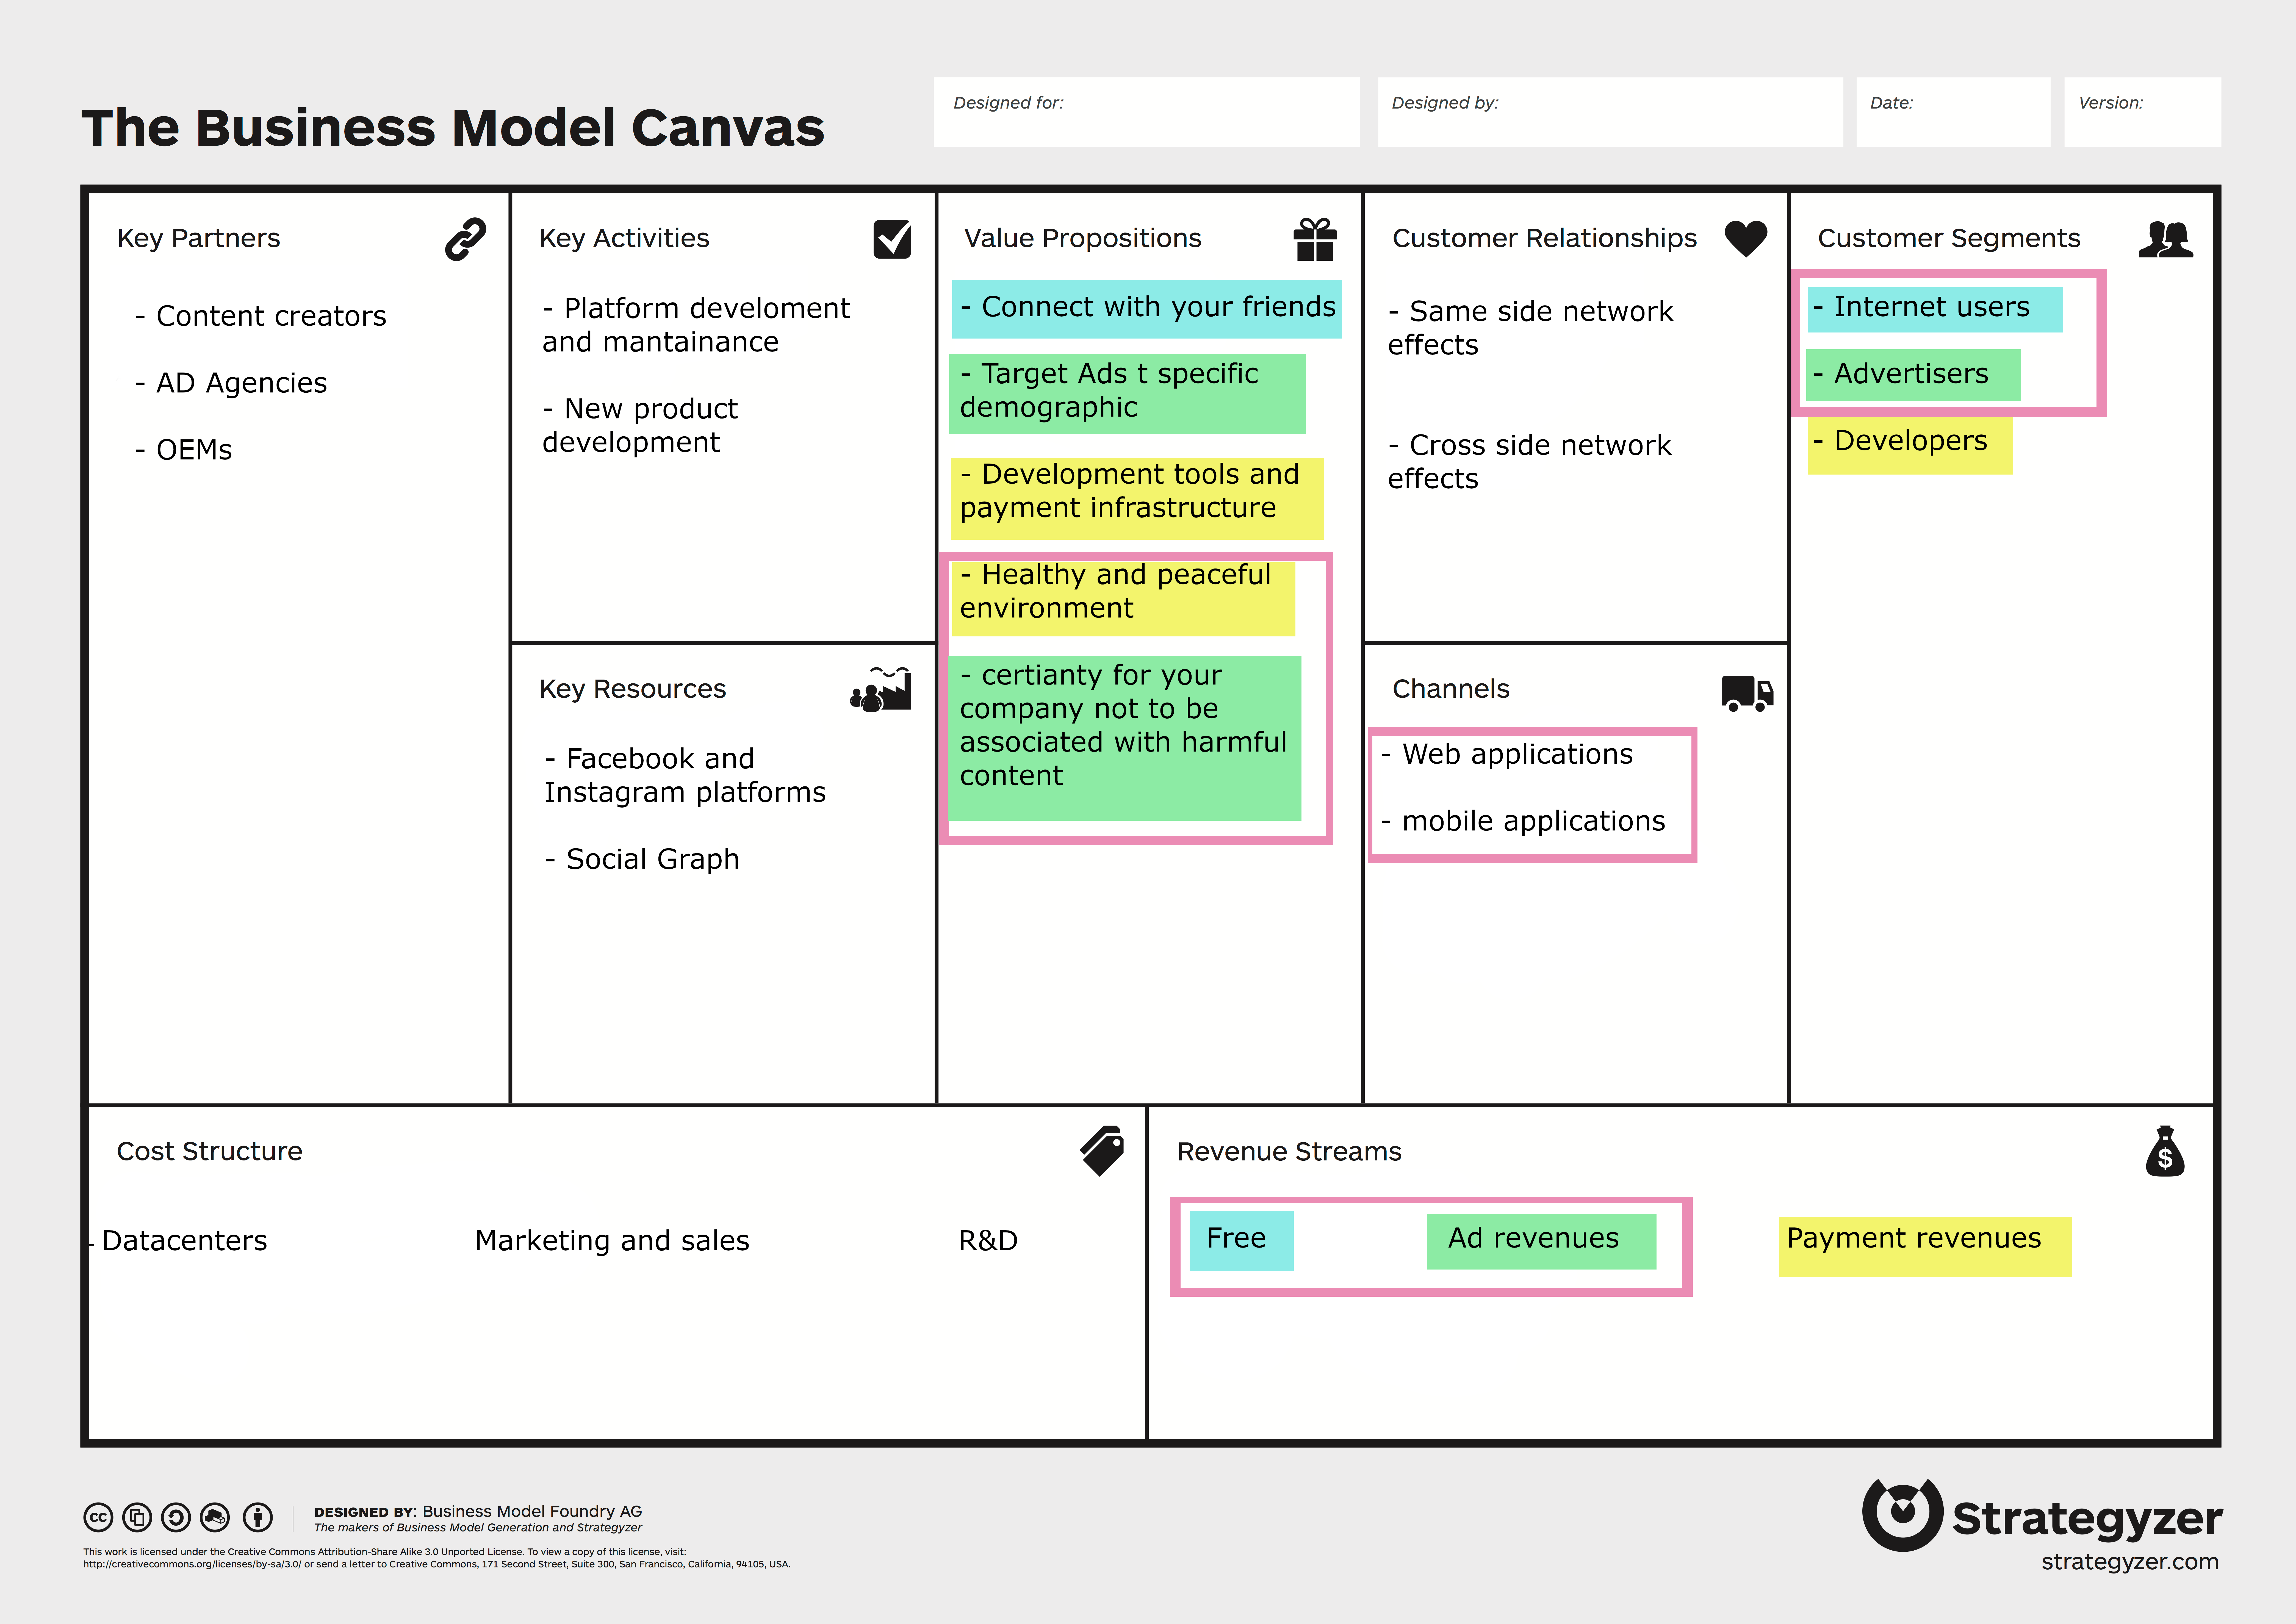
\includegraphics[width=.8\textwidth]{images/newcanvas}
  \caption{new value propositions in the business model due to
    innovations in the AI recognising hate speech, source: author's
    elaoration.}
  \label{fig:newcanvas}
\end{figure}

In red in the figure \ref{fig:newcanvas} we can see what targets and
channels the innovation tackles, along with what new value proposition
it offers to users and advertisers. The main point on wich this
technology operates is the relationship between the users and the
platform, and between the platform and the advertisers. Both these
categories of customers are crucial to the liveness of the company,
and mantaining a good relationship with them is a core aspect of Meta
business model.
